\chapter{Oplossingen en oplosbaarheid}\label{ch:g6:solutions-and-solubility}

Er gaat een fles bruisend water open: een gesis, en uit het niets stijgt
een stroom piepkleine belletjes op. Een seconde eerder zag het water er
volkomen helder uit, en toch zat er al die tijd een gas in opgelost.
Vaste stoffen \omterm{def:g2:mixing-and-dissolving:dissolve}{lossen op}, vloeistoffen \omterm{def:g2:mixing-and-dissolving:dissolve}{lossen op}, en ook gassen \omterm{def:g2:mixing-and-dissolving:dissolve}{lossen op}
--- maar nooit onbeperkt. Dit hoofdstuk geeft de delen van een oplossing
een naam en meet hoeveel van een stof een vloeistof kan bevatten.

\begin{recall}
Een vaste stof die in water \omterm{def:g2:mixing-and-dissolving:dissolve}{oplost}, verdwijnt uit het zicht en laat de
vloeistof helder; die heldere vloeistof is een oplossing, en wat
opgelost is, zit er nog in (\cref{ch:g2:mixing-and-dissolving}). Een
oplossing is een \omterm{def:g6:pure-substances-and-mixtures:homogeneous}{homogeen mengsel} van \omterm{def:g6:pure-substances-and-mixtures:species}{chemische stoffen}
(\cref{ch:g6:pure-substances-and-mixtures}). Door het water in te dampen,
krijg je de opgeloste vaste stof terug (\cref{ch:g3:separating-mixtures}).
\end{recall}

\begin{omfigure}
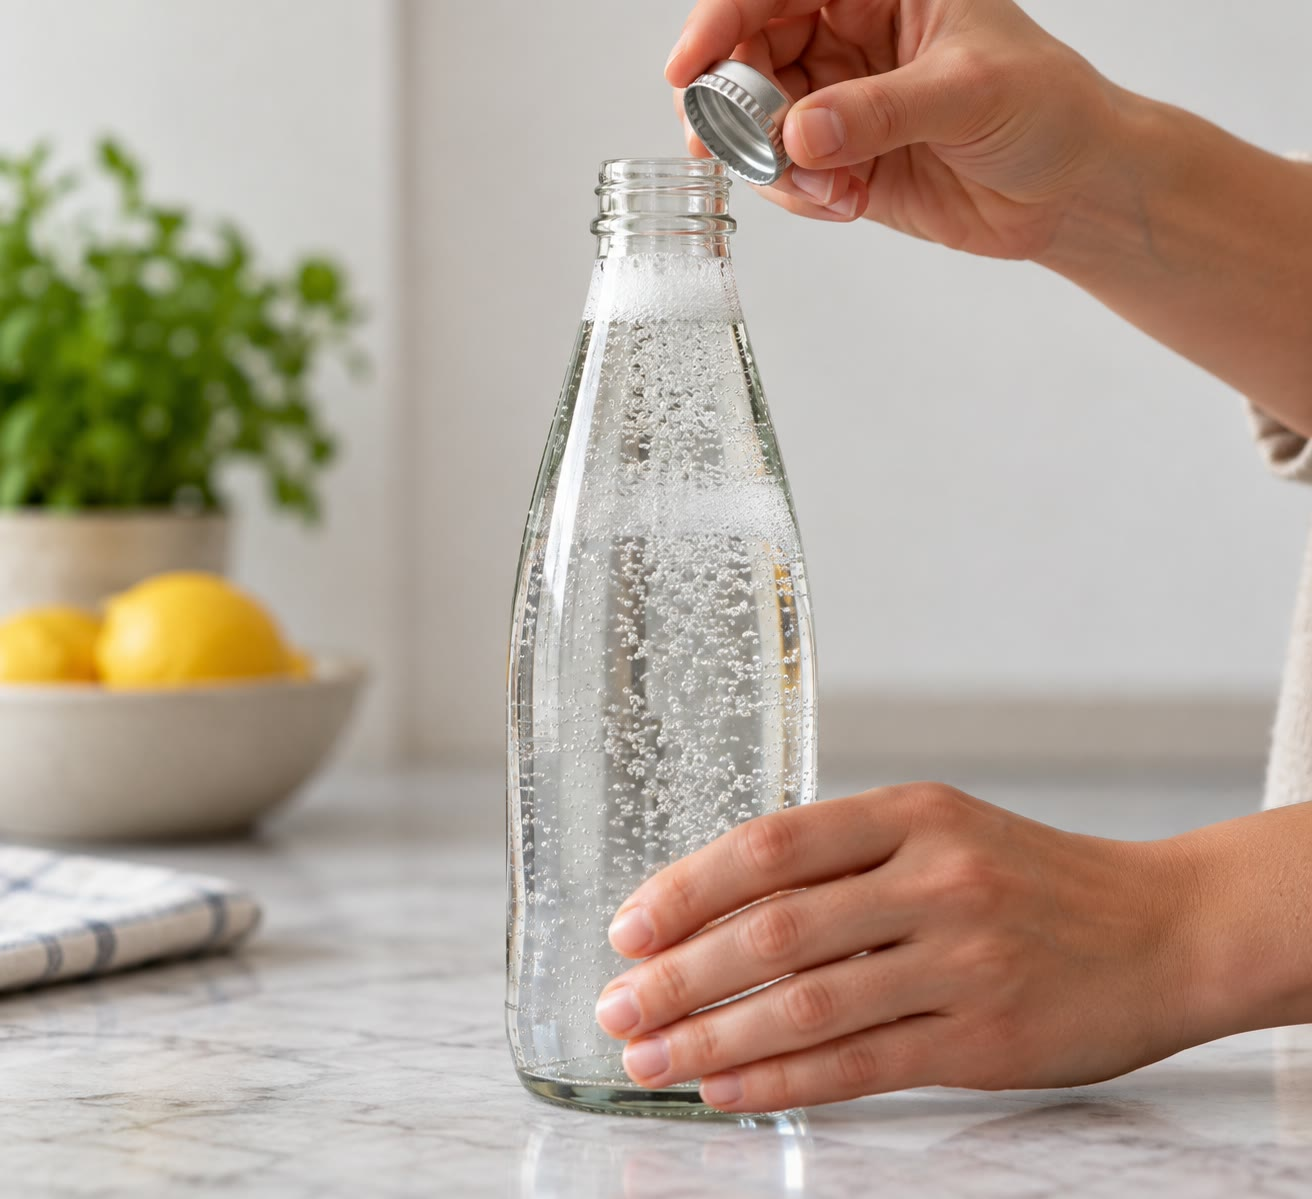
\includegraphics[width=0.5\linewidth]{images/book1/ai/g6-fizzy-water.jpg}

{\small Een fles bruisend water openen: het opgeloste gas komt eruit als
belletjes.}
\end{omfigure}

\section{Opgeloste stof en oplosmiddel}

\begin{definition}[Opgeloste stof, oplosmiddel, waterige oplossing]\label{def:g6:solutions-and-solubility:solute}
In een oplossing heet de stof die \omterm{def:g2:mixing-and-dissolving:dissolve}{oplost} de \emph{opgeloste
stof}\index{opgeloste stof}, en de vloeistof waarin ze \omterm{def:g2:mixing-and-dissolving:dissolve}{oplost} het
\emph{oplosmiddel}\index{oplosmiddel}. Is het oplosmiddel water, dan is
de oplossing een \emph{waterige oplossing}\index{waterige oplossing}.
\end{definition}

\begin{example}[Andere oplosmiddelen dan water]\label{ex:g6:solutions-and-solubility:solvents}
Water is het meest gebruikte \omterm{def:g6:solutions-and-solubility:solute}{oplosmiddel}, maar niet het enige.
Nagellak lost niet op in water; hij \omterm{def:g2:mixing-and-dissolving:dissolve}{lost op} in propanon (aceton), het
\omterm{def:g6:solutions-and-solubility:solute}{oplosmiddel} van nagellakremover. Vet en olieverf \omterm{def:g2:mixing-and-dissolving:dissolve}{lossen op} in
terpentine. Veel geneesmiddelen zijn opgelost in ethanol. Een oplossing
kan meerdere \omterm{def:g6:solutions-and-solubility:solute}{opgeloste stoffen} bevatten: in zeewater zit opgelost zout en
nog veel andere stoffen.
\end{example}

\begin{safety}{\ghs{GHS02}\ghs{GHS07}}
% ledger: ghs:acetone
Propanon (aceton): licht ontvlambare vloeistof en damp (GHS02); het
irriteert de ogen en de damp kan slaperigheid of duizeligheid
veroorzaken (GHS07). Je gebruikt het in een geventileerde ruimte, ver van
elke vlam.
\end{safety}

\begin{proposition}[De massa's tellen op]\label{prop:g6:solutions-and-solubility:mass}
De massa van een oplossing is de massa van het \omterm{def:g6:solutions-and-solubility:solute}{oplosmiddel} plus de massa
van de \omterm{def:g6:solutions-and-solubility:solute}{opgeloste stof}: er gaat niets verloren als een vaste stof \omterm{def:g2:mixing-and-dissolving:dissolve}{oplost},
ook al kun je hem niet meer zien.
\end{proposition}

\begin{omfigure}
\begin{tikzpicture}[font=\small, scale=1.15]
  \pic[transform shape] at (0,0) {balance};
  \pic[transform shape] at (0,0.8) {beaker={0.5}{omWater!80}};
  \node[anchor=north, align=center] at (0,-0.1) {\qty{100}{g} water};
  \node at (1.85,1.3) {$+$};
  \pic[transform shape] at (3.5,0) {balance};
  \fill[white, draw=black!45] (3.0,0.8) rectangle (4.0,0.9);
  \fill[white, draw=black!45] (3.15,0.9) -- (3.85,0.9) -- (3.5,1.2) -- cycle;
  \node[anchor=north, align=center] at (3.5,-0.1) {\qty{10}{g} suiker};
  \draw[->, thick, omProp] (4.9,1.2) -- (6.0,1.2) node[midway, above, text=black]
    {roeren};
  \pic[transform shape] at (7.4,0) {balance};
  \pic[transform shape] at (7.4,0.8) {beaker={0.52}{omWater!80}};
  \node[anchor=north, align=center] at (7.4,-0.1) {\qty{110}{g} suikerwater};
\end{tikzpicture}

{\small Als je \qty{10}{g} suiker \omterm{def:g2:mixing-and-dissolving:dissolve}{oplost} in \qty{100}{g} water, krijg je
\qty{110}{g} oplossing (de massa van het bekerglas is weggelaten).}
\end{omfigure}

\section{Verzadiging en oplosbaarheid}

\begin{definition}[Verzadigde oplossing]\label{def:g6:solutions-and-solubility:saturated}
Een oplossing is een \emph{verzadigde oplossing}\index{verzadigde oplossing}
als ze niets meer van haar \omterm{def:g6:solutions-and-solubility:solute}{opgeloste stof} kan \omterm{def:g2:mixing-and-dissolving:dissolve}{oplossen}: wat je er nog
bij doet, blijft onopgelost op de bodem liggen, hoe lang je ook roert.
\end{definition}

\begin{definition}[Oplosbaarheid]\label{def:g6:solutions-and-solubility:solubility}
De \emph{oplosbaarheid}\index{oplosbaarheid} van een stof in een
\omterm{def:g6:solutions-and-solubility:solute}{oplosmiddel} is de grootste massa van die stof die een gegeven hoeveelheid
\omterm{def:g6:solutions-and-solubility:solute}{oplosmiddel} kan \omterm{def:g2:mixing-and-dissolving:dissolve}{oplossen}, bij een gegeven temperatuur. Voor een vaste
stof in water wordt ze vaak opgegeven in gram per liter (of per
kilogram) water.
\end{definition}

\begin{proposition}[Enkele oplosbaarheden in water]\label{prop:g6:solutions-and-solubility:values}
% ledger: sol:NaCl, sol:sucrose, sol:CO2, sol:O2 (O2: 31 mL/L, 31/24.0 x 32 = 0.041 g/L at 20 C)
Gemeten oplosbaarheden in water lopen enorm uiteen:
\begin{center}
\small
\begin{tabular}{lll}
\hline
\omterm{def:g6:solutions-and-solubility:solute}{opgeloste stof} & \omterm{def:g6:solutions-and-solubility:solubility}{oplosbaarheid} in water & omstandigheden \\
\hline
suiker (sacharose) & ongeveer \qty{2000}{g} per liter water & kamertemperatuur \\
zout (natriumchloride) & \qty{360}{g} per kilogram water & \qty{25}{\celsius} \\
koolstofdioxide & ongeveer \qty{1.5}{g} per liter & \qty{25}{\celsius}, onder het gas \\
zuurstof & ongeveer \qty{0.04}{g} per liter & \qty{20}{\celsius}, onder het gas \\
zand, krijt & vrijwel nul & --- \\
\hline
\end{tabular}
\end{center}
Een liter water kan meer dan zijn eigen massa aan suiker \omterm{def:g2:mixing-and-dissolving:dissolve}{oplossen}, maar
nog geen halve gram zuurstof.
\end{proposition}

\begin{method}[Lost alles op?]\label{met:g6:solutions-and-solubility:will-it}
Om te weten of een massa $m$ van een stof helemaal \omterm{def:g2:mixing-and-dissolving:dissolve}{oplost} in een
volume water:
\begin{enumerate}
  \item zoek de \omterm{def:g6:solutions-and-solubility:solubility}{oplosbaarheid} van de stof op (in g per liter water);
  \item bereken de grootste massa die dit volume water kan \omterm{def:g2:mixing-and-dissolving:dissolve}{oplossen};
  \item vergelijk met $m$: is $m$ kleiner, dan lost alles op; is $m$
        groter, dan is de oplossing verzadigd en blijft de rest op de
        bodem liggen.
\end{enumerate}
\end{method}

\begin{example}[Zout in een glas]\label{ex:g6:solutions-and-solubility:glass}
% ledger: sol:NaCl
Kan \qty{50}{g} zout \omterm{def:g2:mixing-and-dissolving:dissolve}{oplossen} in \qty{200}{mL} water (ongeveer
\qty{200}{g})? Een kilogram water lost hoogstens \qty{360}{g} zout op,
dus \qty{200}{g} water lost hoogstens $360 \times
\frac{200}{1000} = \qty{72}{g}$ op. Omdat $50 < 72$, lost al het zout
op.
\end{example}

\begin{omfigure}
\begin{tikzpicture}[font=\small, scale=1.15]
  \pic[transform shape] at (0,0) {beaker={0.6}{omWater!80}};
  \node[anchor=north, align=center] at (0,-0.15) {een beetje zout:\\ alles opgelost};
  \pic[transform shape] at (3.2,0) {beaker={0.6}{omWater!80}};
  \node[anchor=north, align=center] at (3.2,-0.15) {meer zout:\\ net verzadigd};
  \pic[transform shape] at (6.4,0) {beaker={0.6}{omWater!80}};
  \fill[black!12, draw=black!50] (5.7,0) -- (7.1,0) -- (6.9,0.2) -- (5.9,0.2) -- cycle;
  \foreach \x in {5.85,6.05,6.25,6.45,6.65,6.85} \fill[black!45] (\x,0.09) circle (0.03);
  \node[anchor=north, align=center] at (6.4,-0.15) {te veel zout:\\ de rest blijft onopgelost};
\end{tikzpicture}

{\small Steeds meer zout aan hetzelfde water toevoegen. Zodra de
oplossing verzadigd is, blijft extra zout op de bodem liggen.}
\end{omfigure}

\begin{inthelab}[Zout water verzadigen]
De docent voegt lepel voor lepel zout toe aan \qty{100}{mL} water, en
roert na elke lepel goed. De eerste lepels verdwijnen; dan lost een lepel
niet meer helemaal op en blijven er witte korrels op de bodem liggen: de
oplossing is verzadigd. Als je het gebruikte zout weegt, zie je dat er
ongeveer \qty{36}{g} is opgelost.
\end{inthelab}

\section{Mengbare en niet-mengbare vloeistoffen}

\begin{definition}[Mengbare en niet-mengbare vloeistoffen]\label{def:g6:solutions-and-solubility:miscible}
Twee vloeistoffen zijn \emph{mengbaar}\index{mengbaar} als ze samen
gemengd één enkele homogene vloeistof geven. Ze zijn
\emph{niet-mengbaar}\index{niet-mengbaar} als ze zich in twee lagen
scheiden, de lichtste bovenop.
\end{definition}

\begin{example}[Water met ethanol, water met olie]\label{ex:g6:solutions-and-solubility:liquids}
Water en ethanol zijn \omterm{def:g6:solutions-and-solubility:miscible}{mengbaar}: samen geschud geven ze één heldere
vloeistof. Water en olie zijn \omterm{def:g6:solutions-and-solubility:miscible}{niet-mengbaar}: hoe hard je ook schudt, de
olie komt weer boven en drijft als een aparte laag op het water. In een
pot slasaus drijft de olie boven de azijn, die vooral uit water bestaat.
\end{example}

\begin{omfigure}
\begin{tikzpicture}[font=\small, scale=1.3]
  \pic[transform shape] at (0,0) {testtube={0.6}{omWater!80}};
  \node[anchor=north, align=center] at (0,-0.15) {water + ethanol:\\ één laag};
  \pic[transform shape] at (3,0) {testtube={0.65}{yellow!55!orange!60}};
  \begin{scope}
    \clip (2.75,3) -- (2.75,0.25) arc[start angle=180, end angle=360, radius=0.25]
      -- (3.25,3) -- cycle;
    \fill[omWater!80] (2.7,0) rectangle (3.3,1.1);
  \end{scope}
  \draw[omGlass, line width=0.7pt] (2.75,3) -- (2.75,0.25) arc[start angle=180,
    end angle=360, radius=0.25] -- (3.25,3);
  \draw[<-, omProp, thick] (3.3,1.55) -- (4.1,1.75) node[right, text=black] {olie};
  \draw[<-, omProp, thick] (3.3,0.6) -- (4.1,0.6) node[right, text=black] {water};
  \node[anchor=north, align=center] at (3,-0.15) {water + olie:\\ twee lagen};
\end{tikzpicture}

{\small \omterm{def:g6:solutions-and-solubility:miscible}{Mengbare} vloeistoffen geven één laag; \omterm{def:g6:solutions-and-solubility:miscible}{niet-mengbare} vloeistoffen
geven er twee.}
\end{omfigure}

\begin{omfigure}
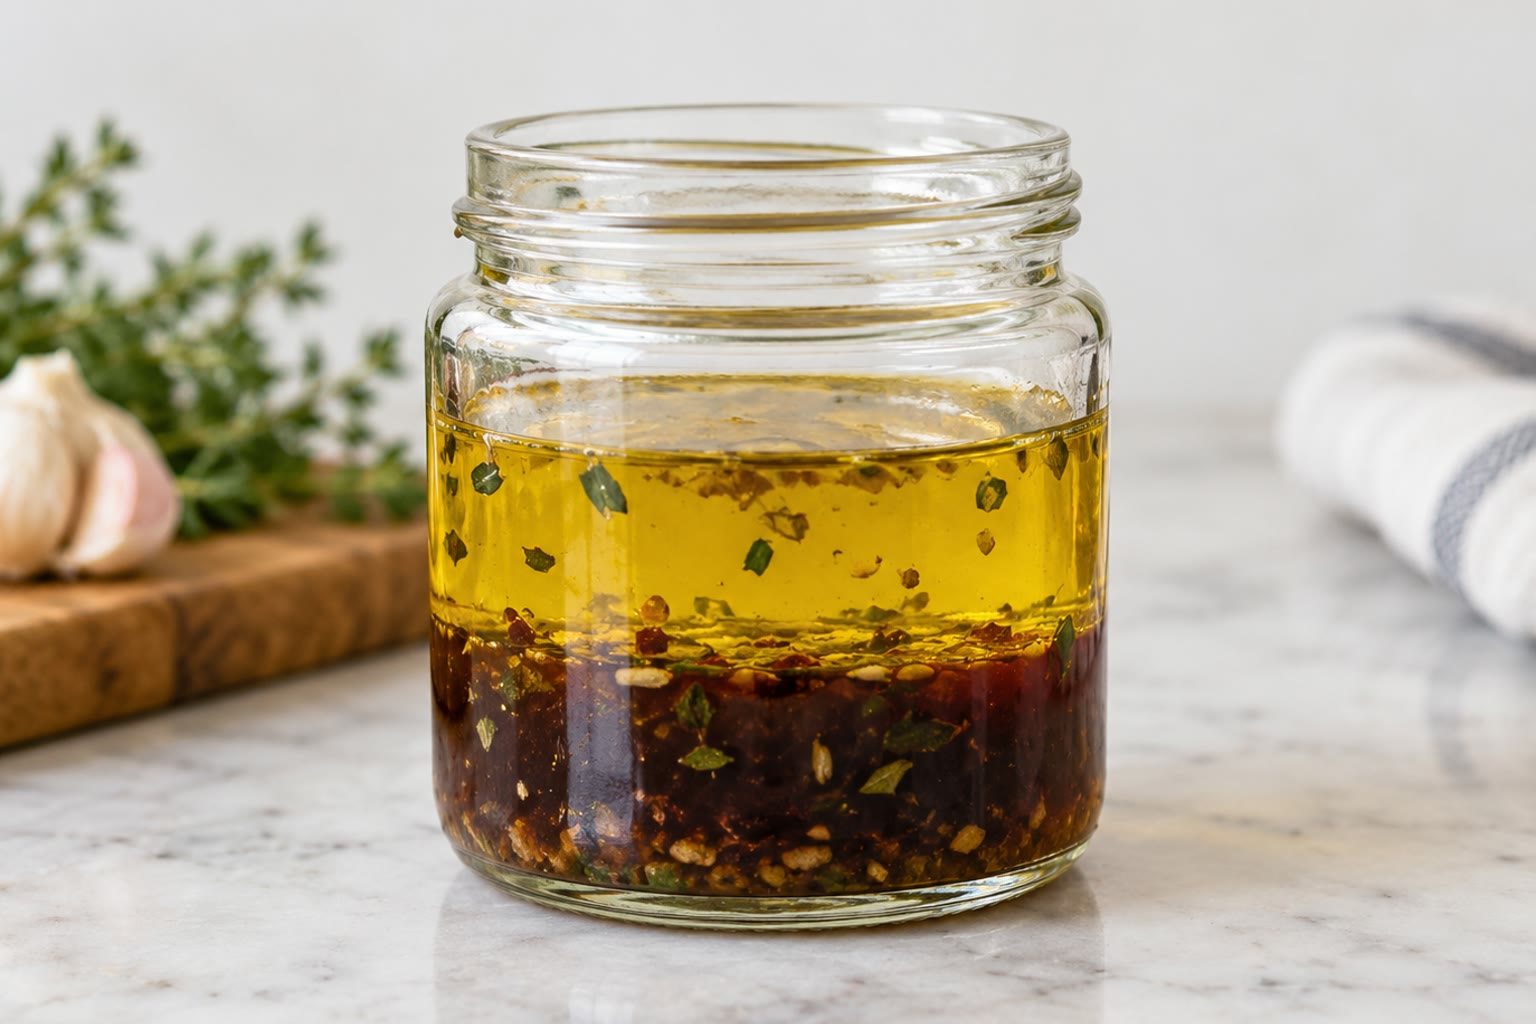
\includegraphics[width=0.45\linewidth]{images/book1/ai/g6-vinaigrette.jpg}

{\small Slasaus: olie en azijn zijn \omterm{def:g6:solutions-and-solubility:miscible}{niet-mengbaar}.}
\end{omfigure}

\section{Ook gassen lossen op}

\begin{proposition}[Opgeloste gassen]\label{prop:g6:solutions-and-solubility:gases}
Gassen lossen een beetje op in water. Bruisende dranken maak je door er
in een gesloten fles onder druk koolstofdioxide in op te lossen; als de
fles opengaat, komt een deel van het gas er weer uit als belletjes.
Water dat met \omterm{def:g4:air-a-mixture-of-gases:air}{lucht} in contact staat, bevat wat opgeloste zuurstof, die
vissen via hun kieuwen opnemen. Een gas lost minder goed op in warm
water dan in koud water: een warme frisdrank verschaalt sneller.
\end{proposition}

\begin{example}[De oceanen en koolstofdioxide]\label{ex:g6:solutions-and-solubility:oceans}
De oceanen staan over twee derde van het aardoppervlak in contact met de
\omterm{def:g4:air-a-mixture-of-gases:air}{lucht}. Koolstofdioxide uit de \omterm{def:g4:air-a-mixture-of-gases:air}{lucht} lost erin op, zodat de oceanen een
deel opnemen van het koolstofdioxide dat mensen in de \omterm{def:g4:air-a-mixture-of-gases:air}{lucht} brengen.
\end{example}

\begin{omfigure}
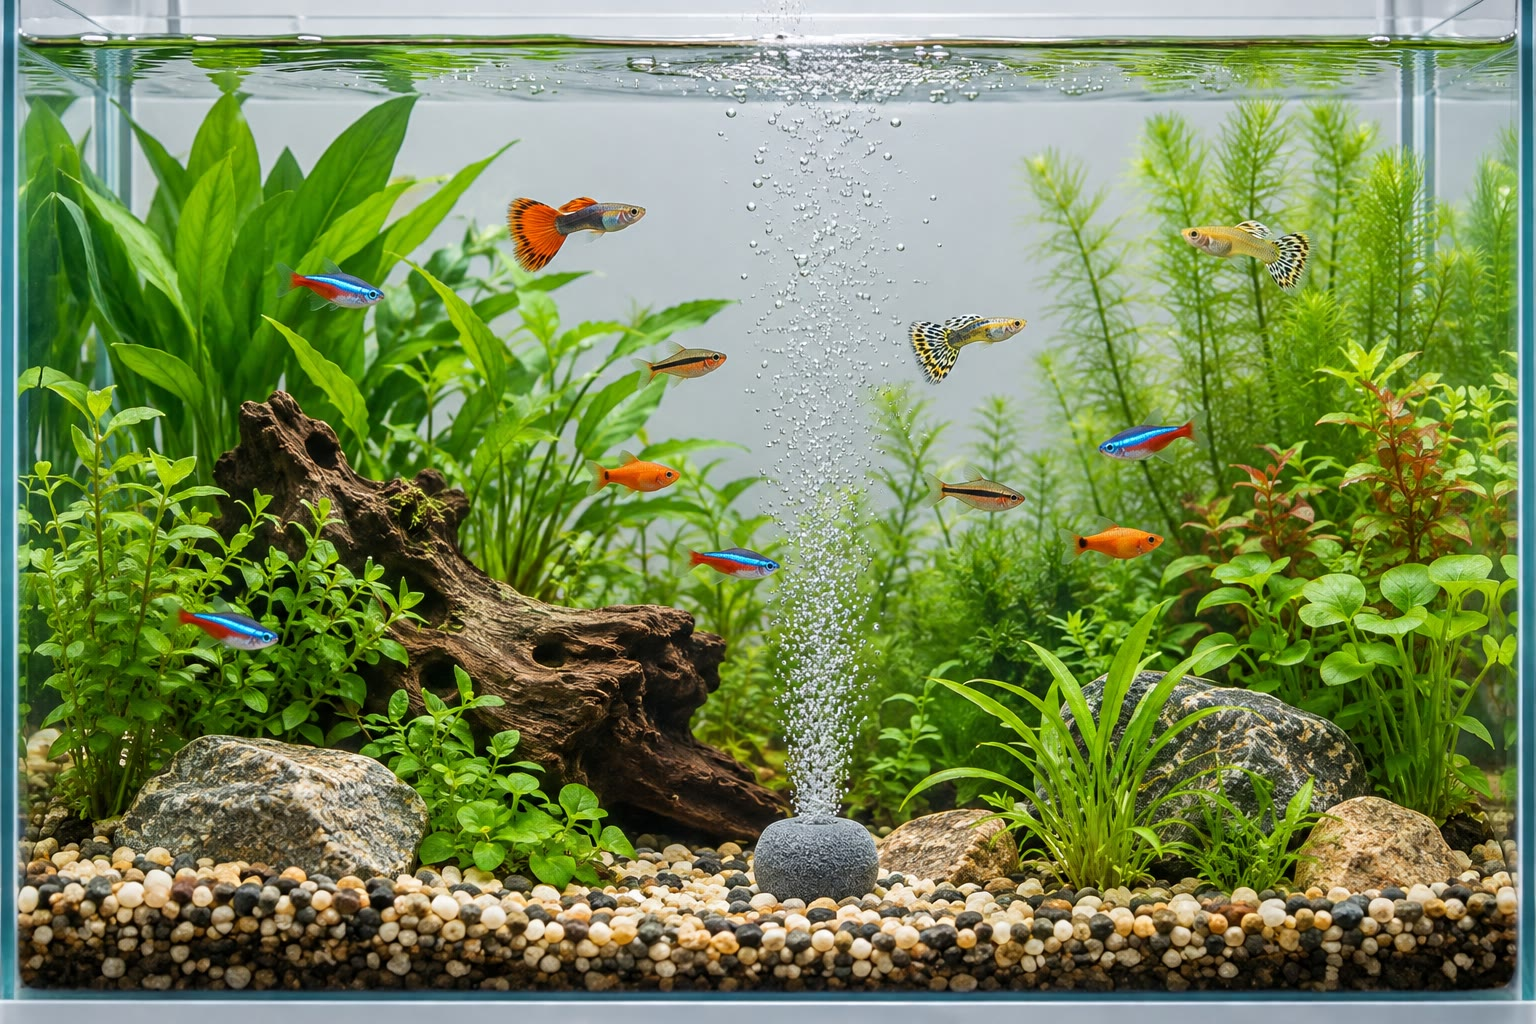
\includegraphics[width=0.5\linewidth]{images/book1/ai/g6-fish-tank.jpg}

{\small Een aquarium: de luchtbelletjes zorgen dat het water opgeloste
zuurstof voor de vissen blijft bevatten.}
\end{omfigure}

\section{Oefeningen}

\begin{exercise}[$\star$]\label{exo:g6:solutions-and-solubility:1}
Noem in suikerwater de \omterm{def:g6:solutions-and-solubility:solute}{opgeloste stof} en het \omterm{def:g6:solutions-and-solubility:solute}{oplosmiddel}. Is het een
\omterm{def:g6:solutions-and-solubility:solute}{waterige oplossing}?
\end{exercise}

\begin{exercise}[$\star$]\label{exo:g6:solutions-and-solubility:2}
Wat is een \omterm{def:g6:solutions-and-solubility:saturated}{verzadigde oplossing}? Hoe kun je zien dat een oplossing
verzadigd is?
\end{exercise}

\begin{exercise}[$\star$]\label{exo:g6:solutions-and-solubility:3}
Er wordt \qty{20}{g} zout opgelost in \qty{250}{g} water. Wat is de
massa van de oplossing?
\end{exercise}

\begin{exercise}[$\star$]\label{exo:g6:solutions-and-solubility:4}
\omterm{def:g6:solutions-and-solubility:miscible}{Mengbaar} of \omterm{def:g6:solutions-and-solubility:miscible}{niet-mengbaar} met water: ethanol, slaolie, azijn?
\end{exercise}

\begin{exercise}[$\star$]\label{exo:g6:solutions-and-solubility:5}
Noem het \omterm{def:g6:solutions-and-solubility:solute}{oplosmiddel} van nagellakremover en geef de betekenis van zijn
twee pictogrammen.
\end{exercise}

\begin{exercise}[$\star\star$]\label{exo:g6:solutions-and-solubility:6}
Bepaal met de \omterm{def:g6:solutions-and-solubility:solubility}{oplosbaarheid} van zout de grootste massa zout die
\qty{500}{g} water bij \qty{25}{\celsius} kan \omterm{def:g2:mixing-and-dissolving:dissolve}{oplossen}.
\end{exercise}

\begin{exercise}[$\star\star$]\label{exo:g6:solutions-and-solubility:7}
Er wordt \qty{80}{g} zout door \qty{200}{g} water van
\qty{25}{\celsius} geroerd. Lost alles op? Zo niet, hoeveel blijft er op
de bodem liggen?
\end{exercise}

\begin{exercise}[$\star\star$]\label{exo:g6:solutions-and-solubility:8}
Er wordt \qty{25}{g} suiker opgelost in \qty{225}{g} water. Welk
percentage van de massa van de oplossing is suiker?
\end{exercise}

\begin{exercise}[$\star\star$]\label{exo:g6:solutions-and-solubility:9}
Kijk naar de figuur van de drie bekerglazen met zout water. In welk
bekerglas kan er nog meer zout \omterm{def:g2:mixing-and-dissolving:dissolve}{oplossen}?
\end{exercise}

\begin{exercise}[$\star\star$]\label{exo:g6:solutions-and-solubility:10}
Waarom bruist een fles bruisend water als je hem opent, en niet
daarvoor?
\end{exercise}

\begin{exercise}[$\star\star\star$]\label{exo:g6:solutions-and-solubility:11}
Een liter water kan ongeveer \qty{2000}{g} suiker \omterm{def:g2:mixing-and-dissolving:dissolve}{oplossen}, maar maar
ongeveer \qty{0.04}{g} zuurstof. Hoeveel keer meer suiker dan zuurstof is
dat?
\end{exercise}

\begin{exercise}[$\star\star\star$]\label{exo:g6:solutions-and-solubility:12}
In de zomer warmt het water van een vijver op en komen de vissen naar
het oppervlak om naar \omterm{def:g4:air-a-mixture-of-gases:air}{lucht} te happen. Leg met dit hoofdstuk uit
waarom.
\end{exercise}

\section{Probleem: De pekel van de kaasmaker}

\begin{problem}[{Weekendprobleem --- een bad verzadigd zout water voor
kazen, en wat de zomerhitte ermee doet}]
\label{pb:g6:solutions-and-solubility:1}
% ledger: sol:NaCl (360 g per kg of water; 1 L of water taken as 1 kg)
Veel kazen liggen een paar uur in een pekelbad: water dat verzadigd is
met zout. Een kaasmaker vult een bak met \qty{20}{L} water
(\qty{20}{kg}) en voegt zout toe tot er wat onopgelost op de bodem
blijft liggen. Neem voor de \omterm{def:g6:solutions-and-solubility:solubility}{oplosbaarheid} van zout \qty{360}{g} per
kilogram water.

\medskip
\noindent\textbf{Deel I --- Woorden.}
\begin{enumerate}
  \item Wat is in de pekel de \omterm{def:g6:solutions-and-solubility:solute}{opgeloste stof}, en wat het \omterm{def:g6:solutions-and-solubility:solute}{oplosmiddel}?
  \item Wat betekent ``verzadigd'' voor de pekel?
  \item Waarom voegt de kaasmaker zout toe tot er een beetje op de bodem
        blijft liggen?
\end{enumerate}

\medskip
\noindent\textbf{Deel II --- De pekel maken.}
\begin{enumerate}[resume]
  \item Hoeveel zout lost er op in de \qty{20}{kg} water?
  \item Wat is de massa van de pekel (zonder het onopgeloste zout)?
  \item Welk percentage van de massa van de pekel is zout? Rond af op
        een geheel getal.
  \item Op een dag wordt er maar \qty{5}{kg} zout toegevoegd. Is de
        pekel verzadigd? Hoeveel zout zou er nog in kunnen \omterm{def:g2:mixing-and-dissolving:dissolve}{oplossen}?
\end{enumerate}

\medskip
\noindent\textbf{Deel III --- Een hete zomer.}
In een hete week verdampt er \qty{5}{L} (\qty{5}{kg}) water uit de
verzadigde pekel van deel II, en er gaat geen zout verloren.
\begin{enumerate}[resume]
  \item Hoeveel water is er nog in de bak?
  \item Hoeveel zout kan dit water nog opgelost houden?
  \item Wat gebeurt er met het zout dat het resterende water niet meer
        kan vasthouden?
  \item Hoe kan de kaasmaker door te kijken zien dat dit gebeurd is?
  \item Bereken de massa zout die op de bodem van de bak is
        uitgekristalliseerd.
\end{enumerate}
\end{problem}
